\section*{Opgave F}

Følgende tre ligheder eftervises:

\begin{enumerate}
    \item $A \cup (B \cap C) = (A \cup B) \cap (A \cup C)$.\\
    
    Ved at skrive lighederne om til udsagnslogik, får vi: 
    \begin{equation*}
        A \vee (B \wedge C) \equiv (A \vee B) \wedge (A \vee C)
    \end{equation*}
    
    Ved at se på logiske ækvivalenser ser vi at dette præcis er reglen for distributivitet af $\wedge$ over $\vee$, givet fra slides i selvstudium:
    
    \begin{figure}[H]
        \centering
        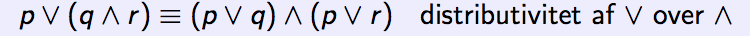
\includegraphics[width=0.7\textwidth]{opgF/WoverV.png}
        \label{fig:WoverV}
    \end{figure}
    
    Lighed 1 er dermed bevist.\\
    \\
    
    \item $A \-- (A \cap B) = A \-- B$. \\
    
    Ved at skrive lighederne om til udsagnslogik, får vi: 
    \begin{equation*}
        A \wedge \neg (A \wedge B) \equiv A \wedge \neg B
    \end{equation*}
    
    Ved at bruge De Morgan-loven: 
    
    \begin{figure}[H]
        \centering
        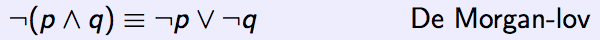
\includegraphics[width = 0.5\textwidth]{opgF/DML1.png}
        \label{fig:DML1}
    \end{figure}
    
    Får vi venstresiden til:
    \begin{equation*}
        A \wedge \neg (A \wedge B) \equiv A \wedge (\neg A \vee \neg B) )
    \end{equation*}
    For at have alle mellemregninger med, bruger vi nu reglen for distributivitet af $\wedge$ over $\vee$:
    
    \begin{figure}[H]
        \centering
        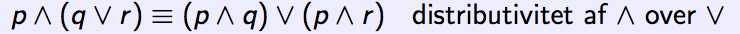
\includegraphics[width=0.7\textwidth]{opgF/VoverW.png}
        \label{fig:VoverW}
    \end{figure}
    
    Dermed får vi: 
    
    \begin{equation*}
        A \wedge (\neg A \vee \neg B) ) \equiv (A \wedge \neg A) \vee (A \wedge \neg B)
    \end{equation*}
    
    Eftersom $A \wedge \neg A$ er en kontradiktion, bliver venstresiden da ækvivalent med:
    
    \begin{equation*}
        (A \wedge \neg A) \vee (A \wedge \neg B) \equiv A \wedge \neg B
    \end{equation*}
    
    Lighed 2 er dermed bevist.\\
    I denne opgave fås en klar forståelse for hvordan mængdedifferensen $A-B$ skal forstås, når $B$ ikke er indeholdt i $A$: Behold elementerne i $A$, fjern elementerne i foreningsmængden.
    
    \item $A \cap ( A \cup B) = A$.

    \textbf{Metode 1}. For at vise at mængdelighed skal vi vise at mængderne er delmængder er hinanden. Dvs. skal vi vise \textbf{3a.} $A \subseteq A \cap ( A \cup B)$ og \textbf{3b.} $A \cap ( A \cup B) \subseteq A$.\\
    \\
    \textbf{3a.} $A \subseteq A \cap ( A \cup B)$ \\
    Betragt et vilkårligt $x$ i $A$: $x \in A$. Så tilhører $x$ også foreningsmængden: $x \in A \cup B$. Da $x$ både tilhører $A$ og $A \cup B$, tilhører $x$ fællesmængden:  $x \in A \cap ( A \cup B)$. Da ovenstående gælder for alle $x$ i $A$, er $A \subseteq A \cap ( A \cup B)$.\\
    \\
    \textbf{3b.} $A \cap ( A \cup B) \subseteq A$\\
    Betragt et vilkårligt $x$ i fællesmængden $A \cap ( A \cup B)$: $x \in A \cap ( A \cup B)$. Da $x$ tilhører fællesmængden, tilhører $x$ både $A$ og $A \cup B$. Dvs. $x \in A$. Da ovenstående gælder for alle $x$ i $A \cap ( A \cup B)$, er $A \cap ( A \cup B) \subseteq A$.\\
    
    \textbf{Metode 2}. Vi oversætter mængdeligheden til udsagnslogik og tjekker med en sandhedstabel. $A \cap ( A \cup B) = A$ oversættes til $A \land (A \lor B) \leftrightarrow A$.
    
    \begin{table}[H]
\centering
\begin{tabular}{c|c|c|c|c}
$A$ & $B$ & $(A \lor B)$ & $A \land (A \lor B)$ & $ A \land (A \lor B) \leftrightarrow A$ \\ \hline
F & F & F & F & T \\
F & T & T & F & T \\
T & F & T & T & T \\
T & T & T & T & T \\
\end{tabular}
\end{table}
    
Det ses at udsagnet $A \land (A \lor B) \leftrightarrow A$ er gyldigt, så $A \cap ( A \cup B) = A$.
    
    % Sprogligt bevis: Antag at $x \in A \cap (A \cup B)$. Da $A \in A \cup B$, da må $x \in A$. Altså må $A \cap (A \cup B) = A$.
    
\end{enumerate}

\begin{figure}[H]
    \centering
    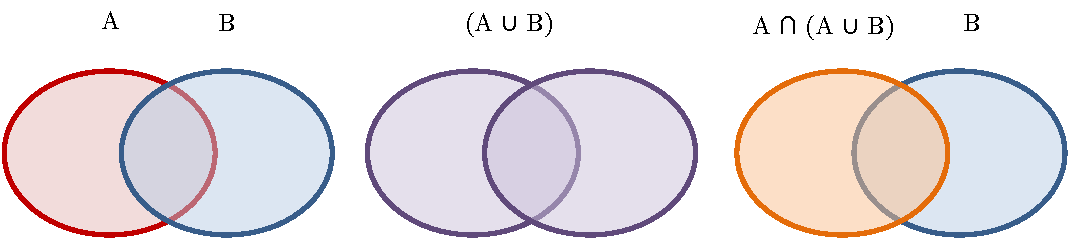
\includegraphics[width=1.0\textwidth]{opgF/F3.pdf}
    \caption{Betragt mængderne  \textcolor{red}{$A$} og \textcolor{blue}{$B$}, og deres foreningsmængde \textcolor{purple}{$A \cup B$}. Alle elementer, der tilhører fællesmængden \textcolor{orange}{$A \cap ( A \cup B)$}, tilhører \textcolor{red}{$A$} (og vice versa).}
    \label{fig:F3}
\end{figure}

